\documentclass[tikz]{standalone}
\usepackage{xcolor}

\begin{document}

\definecolor{COLOR1}{HTML}{6bd2db}
\definecolor{COLOR2}{HTML}{0ea7b5}
\definecolor{COLOR3}{HTML}{0c457d}
\definecolor{COLOR4}{HTML}{ffbe4f}
\definecolor{COLOR5}{HTML}{e8702a}

\usetikzlibrary{decorations.text}

\newcommand*{\mytextstyle}{\sffamily\Large\bfseries\color{black!85}}
\newcommand{\arcarrow}[9]{%
% inner radius, middle radius, outer radius, start angle,
% end angle, tip protusion angle, options, text
  \pgfmathsetmacro{\rin}{#1}
  \pgfmathsetmacro{\rmid}{#2}
  \pgfmathsetmacro{\rout}{#3}
  \pgfmathsetmacro{\astart}{#4}
  \pgfmathsetmacro{\aend}{#5}
  \pgfmathsetmacro{\atip}{#6}
  \fill[#7] (\astart:\rin) arc (\astart:\aend:\rin)
       -- (\aend+\atip:\rmid) -- (\aend:\rout) arc (\aend:\astart:\rout)
       -- (\astart+\atip:\rmid) -- cycle;

    % If flip is active, we switch start and end
    \ifthenelse{\equal{#9}{true}}{
        \pgfmathsetmacro{\tstart}{\aend};
        \pgfmathsetmacro{\tend}{\astart};
    }{
        \pgfmathsetmacro{\tstart}{\astart};
        \pgfmathsetmacro{\tend}{\aend};
    }

  \path[font = \sffamily, decoration = {text along path, text = {|\mytextstyle|#8},
    text align = {align = center}, raise = -1.0ex}, decorate]
    (\tstart+\atip:\rmid) arc (\tstart+\atip:\tend+\atip:\rmid);
}

\newcommand\iterable{
    00/Prediction/COLOR2/true,
    90/Data/COLOR1/true,
    180/Mathematical/COLOR5/false,
    270/Computational/COLOR4/false}

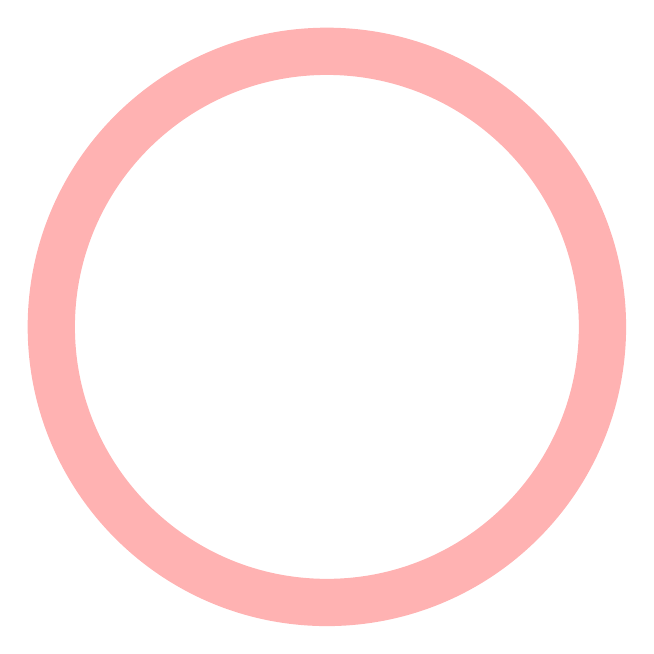
\begin{tikzpicture}
    \fill[even odd rule,red!30] circle (3.8) circle (3.2);
    \foreach \x/\label/\c/\flip in \iterable {
        \arcarrow{3}{3.5}{4}{\x+20}{\x+100}{5}{\c, draw = \c!50!black, very thick}{\label}{\flip}
    }
\end{tikzpicture}
\end{document}
